\documentclass{llncs}


\usepackage{listings}
\usepackage{csquotes}
\usepackage{color}
\usepackage{caption}
\usepackage{graphicx}
\usepackage{zed}
\DeclareGraphicsExtensions{.pdf,.png,.jpg}
%%\newtheorem{definition}{Definition}
 \usepackage{listings}
 \usepackage{courier}
 \lstset{
         basicstyle=\footnotesize\ttfamily, % Standardschrift
         %numbers=left,               % Ort der Zeilennummern
         numberstyle=\tiny,          % Stil der Zeilennummern
         %stepnumber=2,               % Abstand zwischen den Zeilennummern
         numbersep=5pt,              % Abstand der Nummern zum Text
         tabsize=2,                  % Groesse von Tabs
         extendedchars=true,         %
         breaklines=true,            % Zeilen werden Umgebrochen
         keywordstyle=\color{red},
    		frame=b,         
 %        keywordstyle=[1]\textbf,    % Stil der Keywords
 %        keywordstyle=[2]\textbf,    %
 %        keywordstyle=[3]\textbf,    %
 %        keywordstyle=[4]\textbf,   \sqrt{\sqrt{}} %
         stringstyle=\color{white}\ttfamily, % Farbe der String
         showspaces=false,           % Leerzeichen anzeigen ?
         showtabs=false,             % Tabs anzeigen ?
         xleftmargin=17pt,
         framexleftmargin=17pt,
         framexrightmargin=5pt,
         framexbottommargin=4pt,
         %backgroundcolor=\color{lightgray},
         showstringspaces=false      % Leerzeichen in Strings anzeigen ?        
 }
 \lstloadlanguages{
         Java
 }
%\DeclareCaptionFont{blue}{\color{blue}} 

 %\captionsetup[lstlisting]{singlelinecheck=false, labelfont={blue}, textfont={blue}}
 % \usepackage{caption}
 
\DeclareCaptionFont{white}{\color{white}}
\DeclareCaptionFormat{listing}{\colorbox[cmyk]{0.43, 0.35, 0.35,0.01}{\parbox{\textwidth}{\hspace{15pt}#1#2#3}}}
 % \captionsetup[lstlisting]{format=listing,labelfont=white,textfont=white, singlelinecheck=false, margin=0pt, font={bf,footnotesize}}
 
    \graphicspath{{figs/}}
 


\captionsetup[lstlisting]{format=listing,labelfont=white,textfont=white, singlelinecheck=false, margin=0pt, font={bf,footnotesize}}



\begin{document} 

\title{Metadata Registry and management based on ISO11179 using Model Based Engineering}
%If Title is too long, use \titlerunning
%\titlerunning{Short Title}

%Single insitute
\author{David Milward \and Firstname Lastname}
%If there are too many authors, use \authorrunning
%\authorrunning{First Author et al.}
\institute{University of Oxford}
\maketitle

\begin{abstract}
n this paper we present an ISO11179 metadata registry using a data-oriented Domain Specific Modelling Language(DSML). In particular we examine how certain aspects of the ISO11179 specification can be strengthened by using a specific DSML built to handle interoperability use cases, and also how using a model based engineering framework addresses ambiguities in the standard. We examine how the DSML approach taken in this paper presents a concrete realisation of data componentisation, harmonisation, standardisation and reuse of meta-data components. We also examine how the ISO11179 based DSML can be implemented using the Eclipse Modelling Framework and made interoperable with UML In particular, we identify how Model Driven Engineering has helped in achieving the specific goals of ISO11179 via a case study.

\end{abstract}

\keywords{...}

\noindent

\section{Introduction}

ISO11179 is the ISO standard for metadata registries. Metadata registries are used in many organisations to carry out a number of functions, nearly all of them are related to the need to ensure that data is used consistently within an organization.  The need for such a toolkit has become apparent in the last 10 years or so as the amount of data available to organizations has exploded, and despite the existence of an international standard metadata registries are implemented in a variety of different ways. In this paper we look at the intentions of the standard, and since there is no reference implementation of the standard we attempt to build an ISO11179 metadata registry using model driven engineering principles. During this process we examine the strengths and weaknesses of the standard and highlight areas in which the standard can be strengthened, made more user-friendly, adaptable and workable within an enterprise architectural framework. 


\subsection{The Purpose of ISO11179}

The ISO11179 Standard for metadata registries defines its purpose (ISO11179-1 section 0.2 General description of ISO/IEC 11179)as follows,
\newline
to promote:
\begin{itemize}
\item Standard description of data
\item Common understanding of data across organizational elements and between organizations
\item Re-use and standardization of data over time, space, and applications
\item Harmonization and standardization of data within an organization and across organizations
\item Management of the components \emph{of descriptions} of data
\item Re-use of the components \emph{of descriptions} of data.
\end{itemize}

Interoperability isn't specifically mentioned, however these six items are very close to being a description of framework for interoperability for data and data components through the use of \emph{metadata}. There is no other international standards which tackle the issues of interoperability, although there are a number of accepted ``'maturity models' which target interoperability (REF) within the enterprise. These are similar in structure, address similar issues, but diverge slightly on implementation routes. The MDI model framework which emerged from the Athena and Interop NoE (REF) research projects have made progress in defining ways of implementing interoperability using model driven engineering concepts and ideas, and since ISO11179 is currently in use in both the Healthcare and Defence sectors we examine the core purposes of the standard to try and determine how we it achieves these purposes. We implement an ISO11179 conformant metadata registry using Model Based Engineering principles, and examine how use of these principles have helped achieved the purposes of ISO11179. 

****I would like to do the comparison with a strictly conformant MDR such as Aristotle**************

\subsubsection{Standard Data Description}

The standard data description in ISO11179 is given in section1.6.1 where the idea of a data element is introduced, and with it the idea that it is composed of two parts, its conceptual part and its representational part. This section further puts forward the notion that a data element concept can be composed of two parts, an object class and a property. An object class is said to correspond with a class (in OO terms) or an entity(in ER terms). This is further illustrated with the illustration copied below in figure~\ref{fig:DEC}:

\begin{figure}[h]
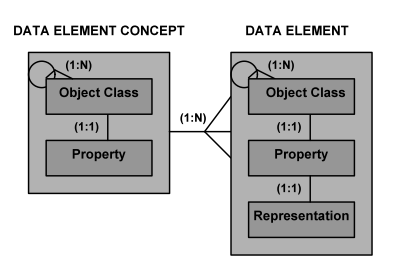
\includegraphics[width=0.6\textwidth,natwidth=610,natheight=642]{DataElementConcept}
\caption{Data Elements and Data Element Concepts} 
\label{fig:DEC}
\end{figure}

The standard continues to describe the relationship between data elements and the concepts associated with them, and also puts forward the notion that a data element is produced when a data element concept is associated with a representation. The notion of \emph{value domains} is introduced, where a value domain is defined as:

\begin{quotation} {sets of permissible values for data} \end{quotation}

  this definition is not very far from the online dictionary of computing definition for the notion of \emph{type}: 
\begin{quotation}
\textbf{type} or \textbf{data type} : A set of values from which a variable, constant, function, or other expression may take its value. A type is a classification of data that tells the compiler or interpreter how the programmer intends to use it. For example, the process and result of adding two variables differs greatly according to whether they are integers, floating point numbers, or strings. 
\end{quotation}

This section then looks in detail at ways in which the conceptual aspects of data elements and value domains are related, and during these discussions the a fundamental model of value domains is presented. Other concepts such as measurement units and enumerations are used to further define the role of the value domain within the standard. Section 1.6 discusses aspects of classification of data elements, apart from the previously introduced notions of object class and property which are part of the Data Element Concept idea. An overview of a metadata registry is introduced in section 1.7, the main feature being that it is a database for metadata built along the lines of the conceptual model provided in section 3 of the standard. Section 1.8 covers the rest of the standard, in addition there is a detailed treatment of terminological principles in the appendix.



\subsubsection{Common understanding of Data}

Part 4 of the standard details how to formulate good data definitions, and data definitions are one of the aspects to achieving a common understanding. The advice in this part of the standard can be summarised as follows: 
\begin{itemize}
\item State the essential meaning of the concept
\item Be precise and unambiguous
\item Be concise
\item Be able to stand alone
\item Be expressed without embedding rationale, functional usage, domain information, or procedural information.
\item Avoid circular reasoning
\item Use the same terminology and consistent logical structure for related definitions
\item Be appropriate for the type of metadata being defined.
\end{itemize}
Use of these guidelines will of course help with the development of a common understanding of data, however it is only when these definitions can be viewed alongside the data item in question that these guidelines can be seen to be useful.


\subsubsection{Re-use and Standardization of Data over time, space and applications}

According to section 5 Standardization involves standardizing the descriptive data itself: characteristics, property values of characteristics, selection of signifiers, and the meaning of values.  It can occur at a variety of levels: agency, national , regional, or international. Governance is further applied by accredited standards organizations, who may well have their own standardization processes. ISO11179-5 details key aspects of naming which should be part of any naming system for data items contained in a registry, and lists a number of criteria which a conforming registry should adhere to. It doesn't prescribe any particular naming system, but rather the key qualities that a naming system should have, and which a registry should document. Part 6 details the organizational requirements for running and administering a metadata registry, however it doesn't specify how re-use or standardization of data over time, space and applications will be enhanced by using an ISO11179 conformant metadata registry. By applying a naming convention to metadata, and by enforcing a rigorous application of that naming convention we can standardise data, however there are no clear practical indications of how this is to be done in the standard.


\subsubsection{Harmonization and Standardization of data}

This is very similar to the purpose of the previous purpose, and again apart from the notes made previously it is difficult to see how the standard itself will further the harmonization of data, apart from the idea of having a uniquely agreed and administered naming and versioning system for data.

\subsubsection{Management of the components \emph{of descriptions} of data}

Here the standard has changed in that the last iteration of the standard has changed the purpose from \emph'{Management of the components of data} to \emph'{Management of the components of descriptions of data}. Most computer scientists would read this as being a change from the idea of \emph{object} to \emph{class}, since an object can be seen as being a component of data, and a class as being a component of a description of data. We consider the term \emph{metadata components} or \emph{models} to be more fitting. Although the management of data components or metadata components is talked about within the standard, it is very often in the terms of the meta-model behind the standard, ideas such as \emph{arranging semantic components with a naming convention} (ISO11179-5.p6) are discussed, but with almost no reference to actual details of what a semantic component is, whether it is referring to combination of a data element and data element concept or an object running in an object oriented programming language. In our view the management models or metadata components is not really addressed by the standard, and it really needs to be.

\subsubsection{Re-use of the components of descriptions of data}

As with the previous discussion we fail to see any direct way in which the standard supports this avowed purpose except indirectly. There is no real definition on what is being referred to by descriptions of data, except in the discussions over what is metadata, when it appears that metadata is defined as being ``'descriptions of data'. This being the case it begs the question of why this purpose is using the terminology \emph{descriptions of data} instead of \emph{metadata}. 

\subsection{Design of an ISO11179 Metadata Registry}

ISO11179-3 has a detailed account of the registry metamodel and its attributes, and sets out to be relevent to application designers, system architects, and software developers. It uses UML 2.4.1 as a modelling language to describe the main features of a conformant metadata registry, although the standard itself is quite clear in not endorsing any particular environment, database management system, database design paradigm, system development methodology, data definition language, command language, system interface, user interface, computing platform or technology required for implementation. However in ISO11179-3.5 a metamodel is used to describe the information model of a metadata registry, and again the standard is clear that this should not limit the actual implementation technology used. The UML description is split into a number of packages:
\begin{itemize}
\item Basic Package
\item Identification Metamodel
\item Designation and Definition Metamodel
\item Registration Package
\item Concepts Package (Concepts and Classification regions)
\item Binary Relations Package
\item Data Descriptions Package
\end{itemize}
Metadata items are constrained by a set of rules which are described as follows:
\begin{itemize}
\item Rule 1 : A metadata item is  \emph{identified} if has one or more identification associations each with a \emph{Scoped\_Identifier} class.
\item Rule 2 : A metadata item is  \emph{designated} if it has one or more item\_designation associations each with a \emph{Designation} class
\item Rule 3 : A metadata item is \emph{defined} if it has one or more item\_definition associations each with a \emph{Definition} class
\item Rule 4 : A metadata item is \emph{classified} if it has one or more Classification association classes, each with a concept class in a Concept\_System.
\item Rule 5 : A metadata item is  \emph{registered} if it has one or more \emph{submission} associations, each with a Submission\_record class.
\item Rule 6 :  A metadata item is  \emph{administered} if it has exactly one stewardship association with a Stewardship\_Record class - only applies where rule 7 does not apply
\item Rule 7 : A metadata item is \emph{attached} if it has exactly one attachment association with an Administered\_Item class - can only apply in cases where rule 6 does not.
\end{itemize}

The standard continues to provide a detailed account of how metadata items are related within the metadata registry, for the purposes of brevity we will not repeat them all here, but we may refer back to specific parts of the standard where required.


\section{A DSML for ISO11179}

In order to look at the ISO11179 standard from a modelling perspective we need to see how the current normative description and UML diagrams, which make up the ISO11179 model, fit into a MBE architecture. Figure~\ref{fig:mbe1} shows the standard view of abstractions from an MBE viewpoint:

\begin{figure}[h]
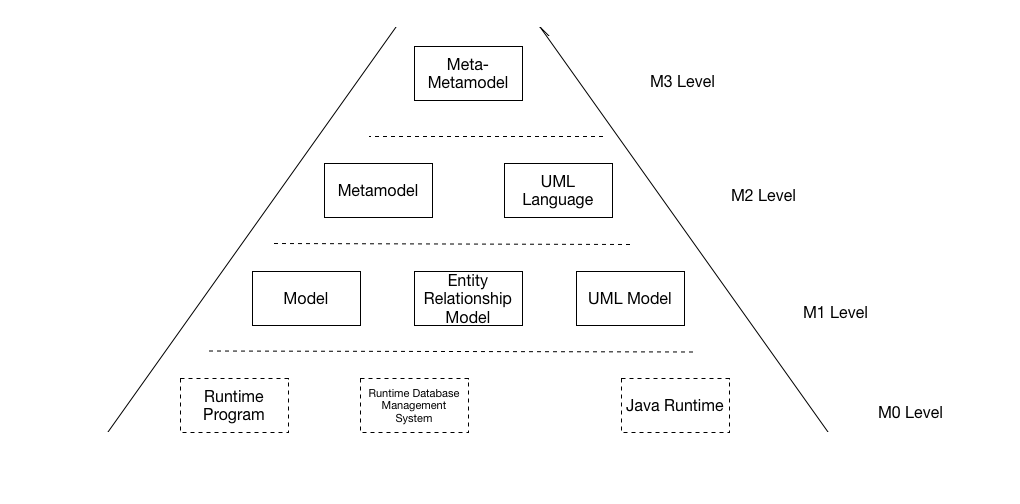
\includegraphics[width=1.0\textwidth,natwidth=610,natheight=642]{Models1}
\caption{Abstraction Layers in Model Based Engineering} 
\label{fig:mbe1}
\end{figure}

In FIgure~\ref{fig:mbe1}  we can see that UML itself sits at what is refered to as the M2 level in this architecture model. Each abstraction layer is defined so that the level \emph{below} can be seen as being an implementation of that layer; in this way the UML model is an implementation of the UML language, which in turn is am implementation of the MOF meta-meta-language which resides at the M3 layer. It is possible to use UML to define meta-models at the M2 level, and this is what is being done here by using UML and text to describe the ISO11179 Model in ISO11179-3. 

The model description in the ISO11179 also defines aspects of the implementation, and no particular regard has been made to differentiating between aspects of the MDR itself, and the groups of metadata which it is holding. In reference to Figure~\ref{fig:mbe1} it is not clear which items belong at M2 and which at M1levels. This makes it quite difficult to implement since it is not always clear from the standard which diagrams pertain to implementation details and which pertain to the core model. In parts of the standard implementation details are deliberately avoided, and in orthers they are clearly indicated. For instance is it necessary to instantiate a class of \emph{Value Domain} objects within the registry, or is it sufficient to represent this aspect of a data element using other properties of a data element.

We have taken the appoach that if we can define the M2 layer, then building the M1 will be straightforward using standard model based engineering techniques. This approach still leaves the implementation details as details which can be adjusted for any particular environment, we can use different code generators on different platforms to generate different implementations of a metadata registry, but still keeping to the original standard.


\subsection{Language Definition}

The metamodel given is informed by experience with Healthcare information systems \cite{DSMCR} and by the development of an open source Metadata Registry built around similar principles. The reason for designing this DSML  is that we seek a meta-language to be able handle hetrogeneous metadata stored using a variety of languages. It needs to be able to capture metadata, in particular a detailed description the data is stored in relational databases, XML Schemas, XML files based on XML Schemas, Excel files and object-oriented programs. It then needs to be able to automatically transform the data into a number of simple formats. To do this each dataset at an M1 level needs to be described at the M2 level, by doing this we can build a container which can hold the metadata collected at the M1 level.

The core entities in the metamodel are as follows:
\begin{itemize}
\item DataModel
\item DataClass
\item DataItem
\item DataType
\item DataConstraint
\end{itemize}

\begin{figure}[h]
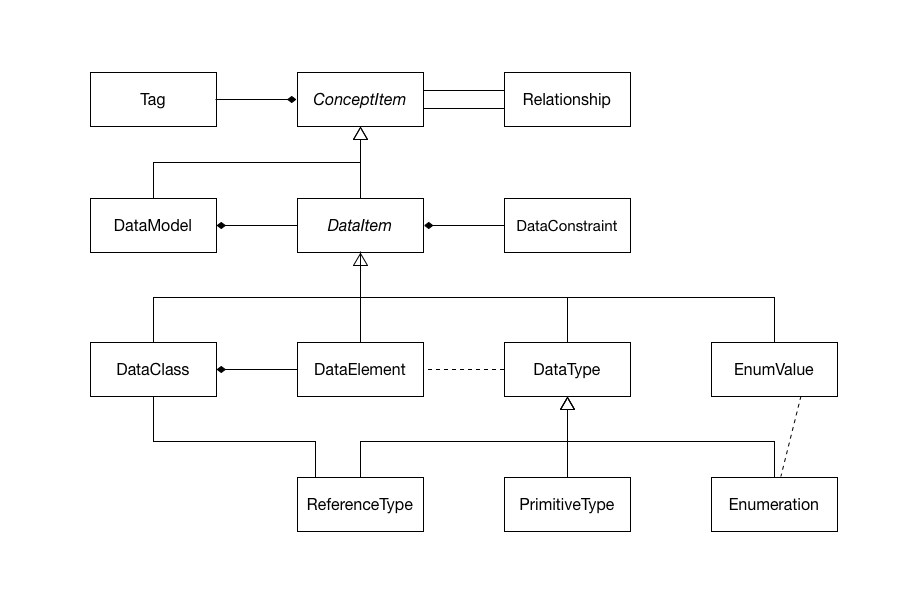
\includegraphics[width=1.0\textwidth,natwidth=610,natheight=642]{LemmaCore1}
\caption{Core Metamodel (Lemma)} 
\label{fig:lemma}
\end{figure}

This metamodel forms a language in its own right which is able to describe the structure of data, it doesn't deal with behaviour so there are no operations in this language, however using the mechanisms inherent in the EMF stack we can define rules which will enable transformations to be defined between LEMMA and for instance a forms metamodel, this is covered inthe next section.

The language is a language of \emph{metadata} and it will normally sit within the context of a metadata registry or similar server artefact. The core entity in our new model is the \emph{CatalogueElement} which is in effect an abstract entities from which most of the other entities derive, it handles the versioning control through the use of a GUID, which has the added benfit of turning metadata into \emph{linked metadata} automatically. The CatalogueElement together with the \emph{Relationship} entity is able to define relationships between any of its sub-entities. The Tag class allows any vocabulary or ontology element to be associated with any catalogue element. This we will see later on will enable the import of standard ontologies into a metadata registry built around this metamodel.

\subsubsection{DataModel}
A DataModel is versioning and grouping mechanism for one data-set, it might for instance be a particular database, or a particular XSD Schema which is used in a particular domain, however it allows us to group and version a related set of DataClasses. A DataModel can contain many DataElements, and many DataTypes. A DataModel contains one or more DataItems, which may be implemented as DataClasses, DataElements, DataTypes or EnumerationValues. As all DataItems are also AbstractItems, they can have Tags, which link them to entities outside that DataModel using URI's, and they can have Relationships which are two-way associations with other AbstractItems. DataConstraints are attached to each DataModel and are applicable within that DataModel.

\subsubsection{DataClass}
 A DataClass is a mechanism for grouping DataItems, which are atomic pieces of data. A concept may be represented by a class, but the DataItem is the atomic component of that class, it can't be reduced into any smaller component. A DataClass can be used as a DataItem, in that it can be contained within another DataClass, and so it can be used to provide multi-level grouping within a DataModel. A DataClass can \emph{extend} another DataClass, this \emph{inheritance} mechanism is very straightforward, it allows the child class to have all the member DataItems and DataClasses that are present in the parent. These DataItems and DataClasses are in effect references, so that if the parent class changes then these \emph{inherited} DataItems and DataClasses will be changed as well.
 
 \subsubsection{DataElement}
 A DataElement is the smallest data entity described in this langauge, it has a direct one to one relationship with a DataType, since every DataElement will have a corresponding DataType. 
 
 \subsubsection{DataType}
 A DataType is a basic type or value representation for a particular DataItem, it represents the kind of unit of the DataItem, for instance for it could be a set of values defined by a enumerations, or it could be a number represented by an integer or double DataType. The notion of DataType here is very similar to that which prevails in the Computer Science world and is defined by Pierce  ~\cite{Pierce} as follows:
\textbf{A type system is a tractable synthetic method for proving the absence of certain program behaviours by classifying phrases according to the kinds of values they compute}. 






\subsection{Semantics}


\subsection{ISO11179}



\section{Metadata Registry}

\subsection{}


\section{Metadata Management}



\section{Results}

\subsection{Comparison of Metadata Registries}


\section{Discussion}

 


\newpage

\bibliographystyle{plain}

\bibliography{md11179}


\end{document}  